\section{Tasking}


\subsection{Introduction}
The tasking elements of PEARL are mapped on the Posix thread library 
(\verb|pthread|) as far as possible. 
The pthread-library suffers in Linux from the absence of a \verb|suspend|-call.
Usually this is solved by doing a blocking systemcall in a signal handler and
invoke the corresponding signal.
This solutions works fine as long as no \verb|TERMINATE|-request is
issued to a suspended task. This will cause an abnormal program
termination --- terminating all threads. 


\subsection{Task Control Block}
The task control block is represented by the attributes of the 
task-object. 
The task control block contains a Posix-semaphore to realize atomistic
operations on the tasks state variables.
A mutex appeared not to be sufficient, since
Posix mutex do no implicit reschedule in case of blocking and unblocking.
This would disturb the preemptive priority  paradigma of PEARL.

\subsection{TERMINATE suspended Task}
The task state diagram as discribed in \cite{pearl90} was extended by two
new states 
\begin{itemize}
\item SUSPEND\_PENDING
\item TERMINATE\_PENDING
\end{itemize}
The new task state diagram looks like fig. \ref{taskStatesLinux}.
Suspend and terminate request from other tasks lead to intermediate states.
During the requested tasks progress it calls the method \verb|DO_PENDING| which
finishes the request.

\begin{figure}[pbht]
\begin{center}
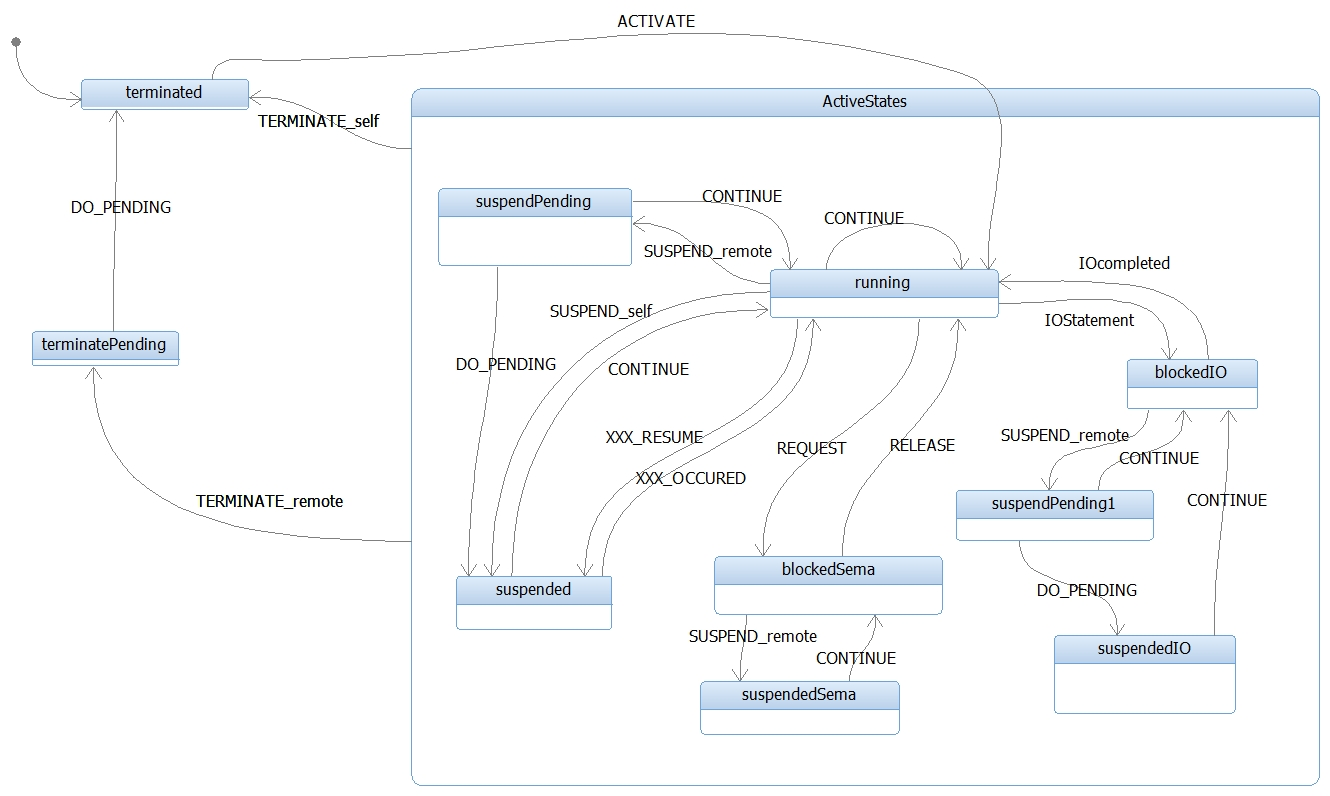
\includegraphics[width=14cm]{../doc_stuff/taskStatesLinux.jpg}
\end{center}
\caption{Extended task state diagram to enable the termination of a 
         suspended task}
\label{taskStatesLinux}
\end{figure}

\paragraph{SUSPEND:}
Depending of the caller of the invocation of \verb|SUSPEND| the behavior
is different:
\begin{description}
\item[from other task] will set the tasks state to \verb|SUSPEND_PENDING|. 
   The task will continue running until the next source line is reached. 
   Inside the method \verb|setLocation(...)| the tasks state is checked for
   any pending state transitions. If there are pending transitions they will 
   be executed.
\item[from own task] will cause a \verb|read|-operation on a pipe. This
   will block the tasks execution immediatelly until a continue is performed
   --- as required by the specification.
\end{description}

This solution modifies the semantic of PEARL programs:
\begin{enumerate}
\item SUSPEND calls on other tasks return before the other taks is really 
    suspended
\item a new task state exists
\end{enumerate}
These changes should not cause trouble for real PEARL applications, since
the continuation of a task which is in the \verb|SUSPEND_PENDING| state
will remove the pending request and the task will go on with the execution.

\paragraph{TERMINATE:}
Depending of the caller of the invocation of \verb|TERMIANTE| the behavior
is different:
\begin{description}
\item[from other task] will set the tasks state to \verb|TERMINATE_PENDING|. 
   The task will continue running until the next source line is reached. 
   Inside the method \verb|setLocation(...)| the tasks state is checked for
   any pending state transitions. If there are pending ransitions they will 
   be executed.
\item[from own task] will terminate the thread immediatelly ---
   as required by the language report.
\end{description}

This solution modifies the semantic of PEARL programs:
\begin{enumerate}
\item TERMINATE calls on other tasks return before the other taks is really 
    terminated
\item a new task state exists
\item the (re-)activation of a task being in the \verb|TERMINATE_PENDIG| 
   state will cause a task running signal. 
\end{enumerate}

This solution provides a behavior that is suitable for PEARL applications.
The foreign termination should only be performed in emergency situations.
In this case, the emergency task may continue performing its operations
without the need of waiting for the real termination of a task.


These changes should not cause trouble for real PEARL applications, since
the continuation of a task which is in the \verb|SUSPEND_PENDING| state
will remove the pending request and the task will go on with the execution.


\subsection{SUSPEND/TERMINATE during I/O-operation}
The i/o-operations are protected by a mutex to enshure the atomistic 
operation of a PUT/GET/READ/WRITE/TAKE/SEND on a specific dation.
In case of terminating a task during an i/o-operation would cause
the mutex to remain in the locked state.
To overcome this problem, there are different solutions possible:
\begin{enumerate}
\item Remove the atomistic behavior of i/o-statements. This is possible,
   since this is not explicitly requested in the language report.
   But this would cause a mixing of e.g. output values from diffent
   tasks to systems console. This may be interpreted as wrong application
   structure but it is considered as insecure in situations where the
   output will e.g. steer something.
\item Introduce an additional state \verb|TERMINATE_PENDING|. This state
   is checked at some points of i/o-operation, e.g. \verb|SKIP|.
   This solution is realized.
\end{enumerate}


Suspending a task while it is doing i/o-operations would cause the dations
lock staying locked. Other tasks would block on attempt to access the same
dation. This behavior is considered as not ideal. To overcome this problem
an additional state \verb|SUSPEND_PENDING| is introduced. This state is
checked at some points of the i/o-operation, e.g. \verb|SKIP|. This will
unlock the mutex and lock again after the continuation.

\subsection{Scheduled Operations (class TaskTimer)}
The scheduled operations like \verb|AFTER ... ACTIVATE| are realized with
Linux timers and realtime signals. 
The timers provide a start delay and repetition rate. This fits ideal to
the \verb|AFTER ... ALL ...| semantics.
The element \verb|AT| ist translated into \verb|AFTER| with respect of the current
time (\verb|NOW|).
The elements \verb|DURING| and \verb|until| are translated into a repetion 
counter. Each time the timer elapses a realtime signal is emitted.
The signal handler is treated inside the timer thread.
The handler decrements the counter.
When the counter reached 0, the timer will be stopped.

The real-time signals have the advantage that the reception is guaranteed.

There are independent timers for \verb|ACTIVATE|, \verb|CONTINUE| 
and \verb|RESUME|.

\paragraph{Remark:} Subsequent modification of the systems date and time 
will not affect the scheduled operation using \verb|AT| or \verb|UNTIL|.

%\subsection{TaskList-class}
%The os-module provides a small command line interface for diagnosis.
%For this reason a list of all tasks is needed.
%The class {\em TaskList} provides a container for all defined tasks.
%The container is implemented using a STL-vector. The STL-vector uses
%dynamic memory allocation. This is in contradiction to the requirement 
%of not using any dynamic memory allocations. But a time of system startup 
%this is not critical.
%
%The PEARL language requires no list of tasks.
%
%\paragraph{Remark:}
%As soon as a module linker utility is available, this list shall be
%replaced by a static array of pointers.
%
%\subsection{TaskMonitor-class}
%Linux is a desktop operating system. Linux applications are expected to end
%after the last possible action occured.
%Emdedded applications run usually eternally.
%
%The module {\em TaskMonitor} provides methods ({\em increment} 
%and {\em decrement}) to monitor the activity 
%of all tasks. Each task informs the TaskMonitor about it operation.
%This behaviour is implemented in the  {\em Task.cc}-module.
%
%\begin{description}
%\item[increment] is executed
%   \begin{itemize}
%   \item  if a task is activated and no scheduled activate 
%   is set for this task
%   \item if a scheduled activate is set and the task not currently not active
%   \end{itemize}
%\item[decrement] is executed
%   \begin{itemize}
%   \item  if a task terminates and no scheduled activate is set for this task
%   \item if a scheduled activate is cancelled and 
%         the task not currently not active
%   \end{itemize}
%\end{description}

\subsection{PrioMapper}
The Linux-scheduler {\em SCHED\_RR} supports 100 priorites. PEARL requieres 
256 different priorities.
The module {\em PrioMapper} maps PEARL-priorities to system priorities as good
as possible. The strategy is to map the best priorities in a 1:1 manner and the
worst priority to 99. 
Request with PEARL-priorities, which are not mappable result in a PEARL
signal raising.

If a different behavior is desired this module can be replaced or modified.


